\documentclass[12pt,oneside,openany,a4paper, %... Layout
afrikaans,english,
%... Global lang drivers
]{memoir}
\usepackage[report, goldenblock]{usthesis}%... Thesis options
\usepackage[afrikaans, english]{babel}

\usepackage{amsmath}
\usepackage{mathtools}
\numberwithin{equation}{chapter}
\usepackage{bm}
\usepackage{graphicx}
\usepackage{color} % or xcolor
\usepackage{float} %figure location

%Watermark
\usepackage{eso-pic}
\newcommand*{\WaterMark}[2][0.15\paperwidth]{%
\AddToShipoutPicture*{\AtTextCenter{%
\parbox[c]{0pt}{\makebox[0pt][c]{%
\includegraphics[width=#1]{#2}}}}}}

%References
\usepackage{usbib}%............................. Bibliography
\bibliographystyle{usmeg-a}%................. Auhor-year style
\addto{\captionsafrikaans}{\renewcommand{\bibname}{Lys van Verwysings}}
\addto{\captionsenglish}{\renewcommand{\bibname}{List of References}}

\begin{document}

%TiltePage:
\title{Numerical integration for probabilisitc reasoning skripsie}
\author{JM.\ Louw}{Jacobus Martin Louw}
\faculty{Faculty of Electrical and Electronic Engineering}
\degree{BEng (E&E)}{Bachelor of Engineering (Electrical and Electronic)}
\ReportDescript{Final Report}
\supervisor{Dr.\ CE\ van Daalen}
\frontmatter
\WaterMark{UScrest-WM}
\TitlePage

%Declaration Page
\DeclarationPage

%abstract
\address{Department of Electrical and Electronic Engineering,\\
University of Stellenbosch,\\
Private Bag X1, 7602 Matieland, South Africa.}
\begin{abstract}
Text in default language ...
\end{abstract}

\chapter{1 Introduction}
For modern mobile vehicles and robots it is important to have the ability to navigate their environment. It is usually critical for these devices to avoid collisions or dangerous environments. Some robots must move very precisely and therefore should have an accurate reading of their location.

Localisation is essential for robot navigation, but is used in various other applications such missile tracking. For applications like this, it is crucial to have accurate and instantaneous information of the missile's location in space. Measurements of any object's location will always have some noise, therefore the measured location is never 100\% accurate. Therefore, one should rather approach the localisation problem in a probabilistic manner. A probability density region where the object is most likely can be calculated.

For systems with continuous random variables, most of the operations used in probabilistic reasoning use integration. These integrals can be solved analytically in the case of a problem with linear movement. Most systems are unfortunately nonlinear. The integrals in nonlinear systems cannot be computed analytically and one has to resort to numerical methods. Commonly-used techniques such as the extend or unscented Kalman filters use rudimentary numerical integration that are very inaccurate in some scenarios. There are several numerical techniques available that are more accurate.

The end goal of this project is to compare different numerical techniques to solve the nonlinear localisation problem. To reach the end goal, one should first have a good understanding of Gaussian random variables and traditional techniques such as the extended - and unscented kalman filters. Modeling the problem with Probabilistic Graphical Models has a lot of advantages and is therefore also investigated. 

A relevant problem has been simulated in Python. Different techniques were implemented and compared in terms of accuracy and efficiency.

\chapter{2 Gaussian Random Variables}
\setcounter{chapter}{2}
The Gaussian or normal distribution is commonly used in probability theory, as it is easy to work with and very close to real-world distributions. Gaussians make strong assumptions such as exponential decay of the distribution away from its mean and linear interactions between variables. Gaussians are in many cases a good approximation for real world distributions, such as noise, even though they make invalid assumptions. The Gaussian random variable (RV) is a very important concept in this paper as all probability distributions are approximated as Gaussian distributions. Key concepts and features of the Gaussian RV are discussed in this chapter. The canonical form and conditional distributions are very important concepts and will be used in following chapters.

\section{2.1 Covariance Form}
\subsection{2.1.1 Univariate Gaussians}
An univariate Gaussian random variable $X$ with mean, $\mu$, and variance, $\sigma^2$, is denoted
\begin{equation}\label{eq:1}
p(x) = \mathcal{N}(\mu;\sigma) = \eta\exp\left[\frac{-(x-\mu)^2}{2\sigma^2}\right]
\end{equation}

\begin{equation}\label{eq:2}
\eta = \frac{1}{\sqrt{2\pi\sigma^2}}
\end{equation}
The mean parameter $\mu$ describes the location of the peak of the distribution and the variance parameter $\sigma^2$ describes the tempo which the distribution decays. The standard deviation is denoted by $\sigma$. The probability of $x$ decays exponentially as $x$ moves farther from the mean. Figure \ref{fig:gPDF1} shows the PDF of three univariate Gaussian distributions. 

\begin{figure}[H]
  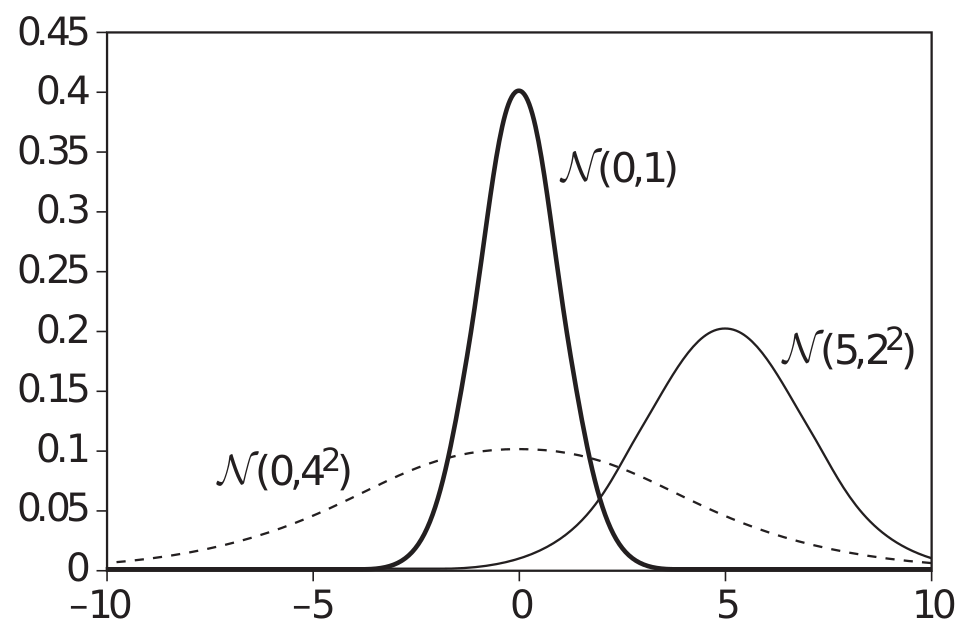
\includegraphics[width=0.7\linewidth]{Figures/PDF_3_Gaussian_Distributions.png}
  \centering
  \caption{PDF of three Gaussian PDFs}
  \label{fig:gPDF1}
\end{figure}

\subsection{2.1.2 Multivariate Gaussians}
The multivariate Gaussian distribution is described by an $n$-dimensional mean vector, $\mu$, and an $n\times n$ covariance matrix. The multivariate Gaussian distribution is commonly described by the following function, where $\eta$ is a normalisation coefficient.
\begin{equation}\label{eq:3}
p(x) = \mathcal{N}(\bm{\mu};\Sigma) = \eta\exp\left[-\frac{1}{2}(\bm{x}-\bm{\mu})^T\Sigma^{-1}(\bm{x}-\bm{\mu})\right]
\end{equation}
\begin{equation}\label{eq:4}
\eta = \frac{1}{(2\pi^{n/2)}|\Sigma|^{\frac{1}{2}}}
\end{equation}
$|\Sigma|$ is the the determinant of $\Sigma$
It is important that the determinant of $\Sigma$ is nonzero for the equation above to be valid. Therefore it is a requirement that $\Sigma$ is positive definite and therefore also non-singular, which guarantees a  determinant that is nonzero. In this paper we focus on positive definite covariance matrices, as it is invertible and therefore one can use the alternative canonical or information parameterization.\\
The mean and covariance can be found by sequentially calculating the first and second moments of the Gaussian distribution.\\
The mean corresponds to the first moment:
\begin{equation}
\bm{\mu} = \bm{E}\left[\bm{X}\right]
\end{equation}
The covariance corresponds to the second moment:
\begin{equation}
\bm{\Sigma} = \bm{E}[\bm{XX}]^T - \bm{E}[\bm{X}]\bm{E}[\bm{X}]^T
\end{equation}
\subsection{2.1.3 Error Ellipse}
Multivariate Gaussian distributions can be visualized as a series of ellipsoidal contours around the mean vector $\bm{\mu}$. The contours are parallel to each other and the distance between contours suggests the steepness of the density function. The steepness of the density function is determined by the covariance matrix $\Sigma$.\\
Plotting the error ellipses is an effective way to illustrate the distribution

\section{2.2 Canonical Form}
Linear Gaussian CPDs (conditional probability densities) are conditional distributions and are generally not Gaussians. It will be handy to find general representation that accommodates both Gaussian distributions and linear Gaussian models. The canonical or information form is a viable option. It is also much easier to perform certain operations in the canonical form. 

\begin{equation}\label{eq:5}
\mathcal{C}(\bm{X}; K,\bm{h},g) = \exp\left(-\frac{1}{2}\bm{X}^TK\bm{X} + \bm{h}^T\bm{X} +g \right)
\end{equation}


It is possible to represent every Gaussian as a canonical form. Equation \ref{eq:3} can be rewritten:


\begin{multline}\label{eq:6}
\eta\exp\left[-\frac{1}{2}(\bm{x}-\bm{\mu})^T\Sigma^{-1}(\bm{x}-\bm{\mu})\right]
\\ = \exp\left(-\frac{1}{2}\bm{x}^T\Sigma^{-1}\bm{x} + \bm{\mu}^T\Sigma^{-1}\bm{x} - \frac{1}{2}\bm{\mu}^T\Sigma^{-1}\bm{\mu} + \ln{\eta}\right)
\end{multline}


$\mathcal{N}(\bm{\mu}; \Sigma) = \mathcal{C}(K,\bm{h}, g)$ by comparing \ref{eq:6} with \ref{eq:5}:

\begin{equation}\label{eq:7}
K = \Sigma^{-1}
\end{equation}
\begin{equation}\label{eq:8}
\bm{h} = \Sigma^{-1}\bm{\mu}
\end{equation}
\begin{equation}\label{eq:9}
g = - \frac{1}{2}\bm{\mu}^T\Sigma^{-1}\bm{\mu} + \ln{\eta}
\end{equation}
$\bm{h}$ is called the potential vector and $K$ is called the information matrix.\\\\
The covariance parameters can again be recovered. 
\begin{equation}
\Sigma = K^{-1}
\end{equation}
\begin{equation}
\bm{\mu} = \Sigma\bm{h}
\end{equation}
The covariance form is not defined when K is not invertible, even though the distribution can still be represented in the canonical form. The canonical form is only a valid Gaussian density if and only if $K$ (information matrix) is symmetric and positive definite. The canonical form is therefore more general than the covariance form. The canonical form is very useful to present linear Gaussian CPDs. From \ref{eq:9} it can be seen that only $K$ and $\bm{h}$ are necessary to calculate $g$. Thus, $g$ can be omitted when working in the canonical form. \\


\subsection{2.2.1 Operations using the canonical form}
The main advantage of using the canonical form is that it is very easy to perform various operations on distributions. The variable $g$ is included in the following operations for completeness sake, but can be omitted as stated above.\\

Extending and rearranging scopes of canonical forms may be necessary before doing operations, as it is important that scopes are identical when doing operations.
\paragraph{Extending the scope of a canonical form:}\mbox{}\\
If additional variables are needed, the scope of a canonical form can be extended by adding zero entries to $K$, $\bm{h}$ and $g$. 
\begin{equation}
\mathcal{C}\left(
\begin{bmatrix}
x\\
y
\end{bmatrix}:
\begin{bmatrix}
k_{xx} & k_{xy}\\
k_{yx} & k_{yy}
\end{bmatrix},
\begin{bmatrix}
h_x\\
h_y
\end{bmatrix},
\begin{bmatrix}
g_x\\
g_y
\end{bmatrix}
\right)
=
\mathcal{C}\left(
\begin{bmatrix}
x\\
y\\
z
\end{bmatrix}:
\begin{bmatrix}
k_{xx} & k_{xy} & 0\\
k_{yx} & k_{yy} & 0\\
0 & 0 & 0
\end{bmatrix},
\begin{bmatrix}
h_x\\
h_y\\
0
\end{bmatrix},
\begin{bmatrix}
g_x\\
g_y\\
0
\end{bmatrix}
\right)
\end{equation}
\paragraph{Rearranging the scope of a canonical form:}\mbox{}\\
The order of the scope can be rearranged by rearranging the rows and columns of $K$  and rearranging the entries of $\bm{h}$ and $g$.
\begin{equation}
\mathcal{C}\left(
\begin{bmatrix}
x\\
y\\
z
\end{bmatrix}:
\begin{bmatrix}
k_{xx} & k_{xy} & k_{xz}\\
k_{yx} & k_{yy} & k_{yz}\\
k_{zx} & k_{zy} & k_{zz}
\end{bmatrix},
\begin{bmatrix}
h_x\\
h_y\\
h_z
\end{bmatrix},
\begin{bmatrix}
g_x\\
g_y\\
g_z
\end{bmatrix}
\right)
=
\mathcal{C}\left(
\begin{bmatrix}
y\\
x\\
z
\end{bmatrix}:
\begin{bmatrix}
k_{yy} & k_{yx} & k_{yz}\\
k_{xy} & k_{xx} & k_{xz}\\
k_{zy} & k_{zx} & k_{zz}
\end{bmatrix},
\begin{bmatrix}
h_y\\
h_x\\
h_z
\end{bmatrix},
\begin{bmatrix}
g_y\\
g_x\\
g_z
\end{bmatrix}
\right)
\end{equation}
\paragraph{Multiplication of canonical forms:}\mbox{}\\
When multiplying to canonical forms, it is important that their scopes are identical. Multiplying canonical forms with the same scope is simply:
\begin{equation}\label{eq:10}
\mathcal{C}(K_1,\bm{h_1},g_1)\times\mathcal{C}(K_2,\bm{h_2},g_2) = \mathcal{C}(K_1 + K_2,\bm{h_1} + \bm{h_2},g_1 + g_2)
\end{equation}
\paragraph{Division of canonical forms:}\mbox{}\\
Again, it important that the scopes of the distributions are identical.
\begin{equation}\label{eq:11}
\frac{\mathcal{C}(K_1,\bm{h_1},g_1)}{\mathcal{C}(K_2,\bm{h_2},g_2)} = \mathcal{C}(K_1 - K_2,\bm{h_1} - \bm{h_2},g_1 - g_2)
\end{equation}
\paragraph{Marginalization of a canonical form:}\mbox{}\\
A marginal distribution can be found by integrating over a subset of variables. For example the marginal distribution over $\bm{X}$ can be found by integrating over $\bm{Y}$.\\
Let $\mathcal{C}(\bm{X},\bm{Y};K,\bm{h},g)$ be a canonical form with subsets $\bm{X}$ and $\bm{Y}$ where
\begin{equation}
K = 
\begin{bmatrix}
K_{\bm{XX}} & K_{\bm{XY}}\\
K_{\bm{XY}} & K_{\bm{YY}}
\end{bmatrix}
 ; h = 
\begin{pmatrix}
h_{\bm{X}} \\
h_{\bm{Y}}
\end{pmatrix}
\end{equation}
To obtain the marginal distribution over $\bm{X}$, we have to find the integral over $\bm{Y}$. Therefore
\begin{equation}
\int\mathcal{C}(\bm{X},\bm{Y};K,\bm{h},g)d\bm{Y} = \mathcal{C}(\bm{X};K',\bm{h}',g')
\end{equation}
 where
\begin{equation}
K' = K_{\bm{XX}} - K_{\bm{XY}}K_{\bm{XY}}^{-1}K_{\bm{YX}}
\end{equation}
\begin{equation}
h' = \bm{h}_{\bm{X}} - K_{\bm{XX}}K_{\bm{YY}}^{-1}\bm{h}_{\bm{Y}}
\end{equation}
\begin{equation}
g' = g - \frac{1}{2}\left(\ln|2\pi K_{\bm{YY}}^{-1}|+ \bm{h_Y}^T K_{\bm{YY}}^{-1}\bm{h_Y}\right)
\end{equation}
It is important to that $K_{\bm{YY}}$ is positive definite for the result to be finite.
\paragraph{Reduction with evidence:}\mbox{}\\
Let $\mathcal{C}(\bm{X},\bm{Y};K,\bm{h},g)$ be a canonical form with subsets $\bm{X}$ and $\bm{Y}$. If subset $\bm{Y}$ is known $(\bm{Y} =  \bm{y})$, then the canonical form can be reduced to $\mathcal{C}(\bm{X}; K',\bm{h}',g')$, where
\begin{equation}
K' = K_{\bm{XX}}
\end{equation}
\begin{equation}
h' = \bm{h}_{\bm{X}} - K_{\bm{XY}}\bm{y}
\end{equation}
\begin{equation}
g' = g + \bm{h}_{\bm{y}}^T\bm{y} - \frac{1}{2}\bm{y}^TK_{\bm{YY}}\bm{y}
\end{equation}

\subsection{2.2.2 Using the canonical form the present conditional distributions}

\end{document}\grid
